\chapter{Fundamental Algorithms}
In this chapter, we will go through popular machine learning algorithms. In general, machine learning algorithms that are the basis of artificial intelligence (AI) such as image recognition, speech recognition, recommendation systems, ranking and personalization of content. They aren't generally designed to infer the underlying \textit{generative process} (e.g., to model something), but rather to predict or classify with the most accuracy.

\section{Three Basic Algorithms}
We will first provide you with basic tools to use, so we will start the simple three \textit{linear regression, k-nearest neighbors}, and \textit{k-means}.

\subsection{Linear Regression}
When you use it, you are making the assumption that there is a \textit{linear} relationship between an outcome variable (sometimes also called the response vairable, dependent variable, or label) and a predictor (sometimes also called an independent variable, explanatory variable, or feature); or between one variable and several other variables, in which case you're \textit{modeling} the relationship as having a linear structure.

\begin{tcolorbox}[enhanced jigsaw, breakable, pad at break*=1mm, colback=gray!20!white, colframe=black!85!black, title=\textbf{Algorithm or a Model?}]
    The two words seem to be used interchangeably when their actual definitions are not the same thing at all. In the purest sense, an algorithm is a set of rules or steps to follow to accomplish some task, and a model is an attempt to describe or capture the world.

    To differentiate the two in machine learning, think of an algorithm as a process and a model as the result of running the process. In other words, you use an algorithm to create a model.
\end{tcolorbox}

How to describe something of a linear nature? \(y=f(x)=\beta_{0}+\beta_{1}x\). Let's approach this from the perspective of deterministic function first.

\textbf{Example 1} Suppose you run a social networking site that charges a monthly subscription fee of \$25, and that this is your only source of revenue. Each month you collect data and count your number of users and total revenue. You’ve done this daily over the course of two years, recording it all in a spreadsheet. You could express this data as a series of points. Here are the first four:
$$
    S=\{(x, y)=(1,25),(10,250),(100,2500),(200,5000)\}
$$
If you showed this to someone else who didn't even know how much you charged or anything about your business model (what kind of friend wasn't paying attention to your business model?!), they might notice that there's a clear relationship enjoyed by all of these points, namely \(y=25x\). This is a deterministic function, and it’s a linear one. It's also a perfect fit for the data. If you were to plot it, you'd see that it passes through every point (Fig.\ref{fig:algo_1}).

\begin{figure}[H]
    \centering
    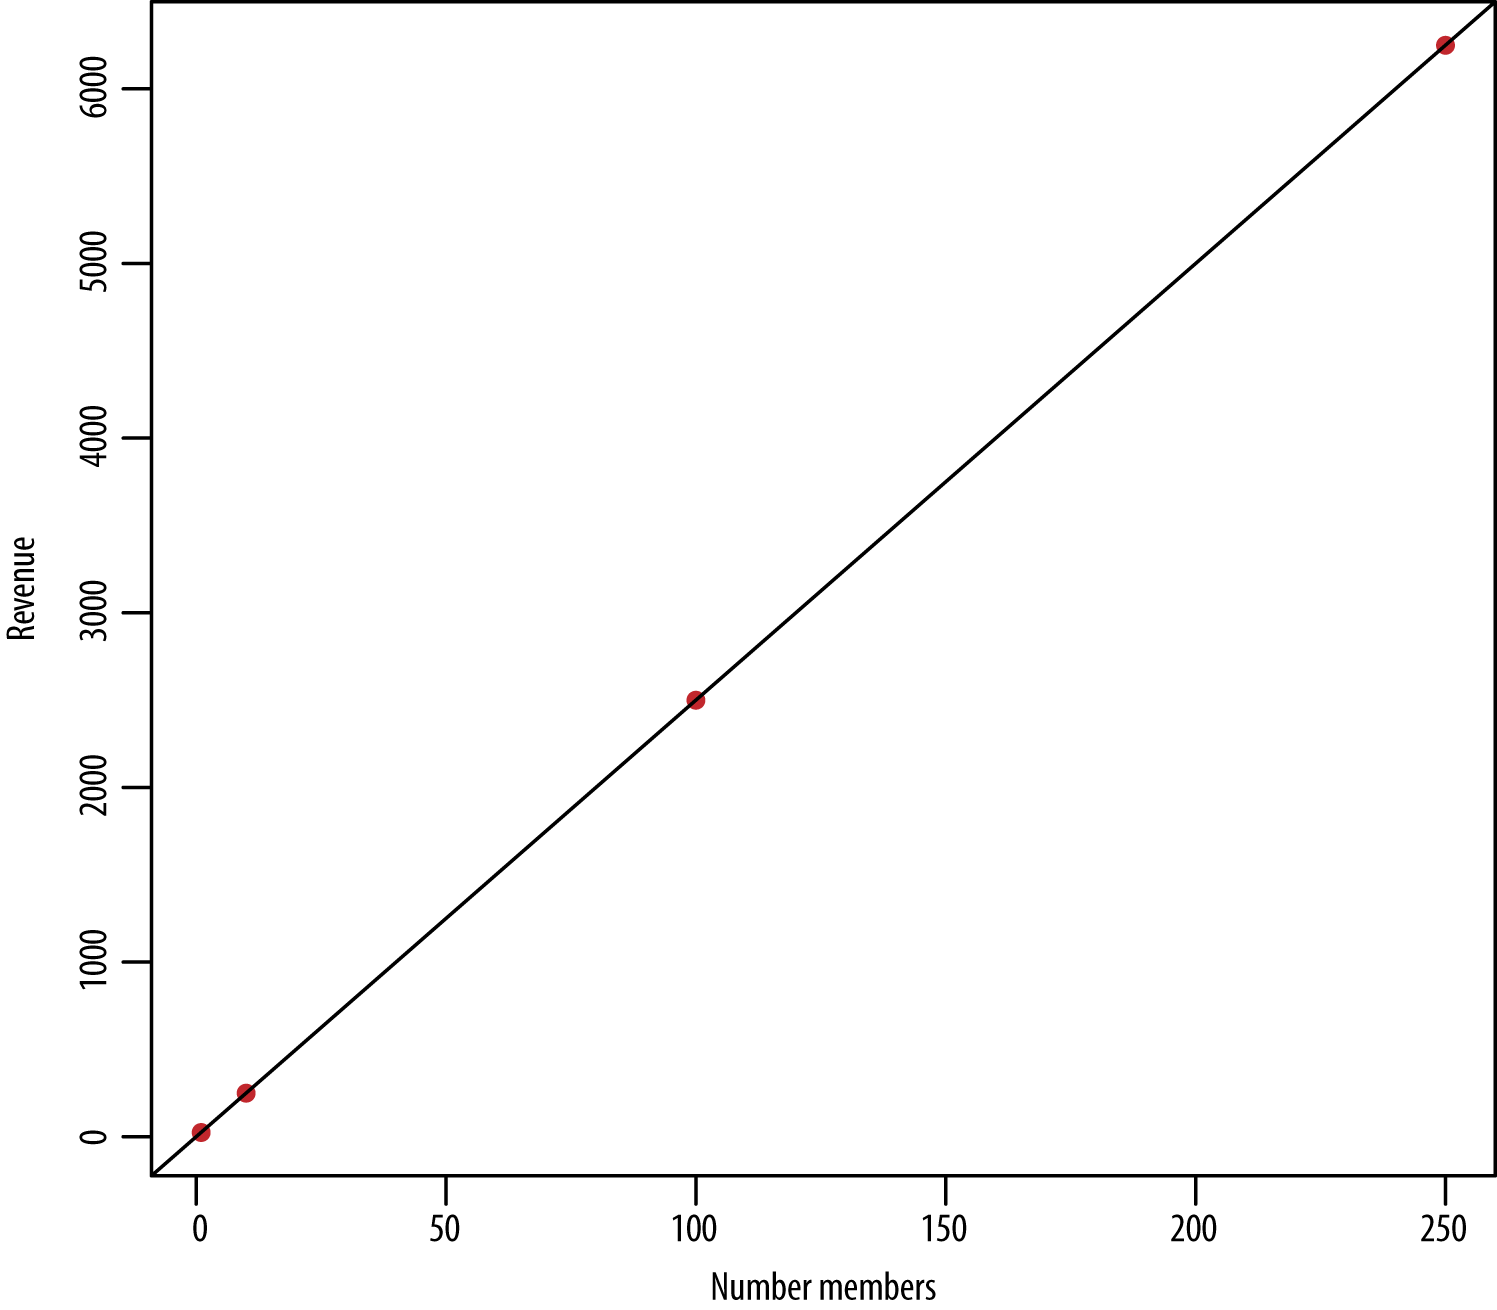
\includegraphics[width=0.7\linewidth]{imgs/fundamental_algo/algo_1.png}
    \caption{An obvious linear pattern}
    \label{fig:algo_1}
\end{figure}

\textbf{Example 2} Say you have a dataset \textit{keyed} by user (meaning each row contains data for a single user), and the columns represent user behavior on a social networking site over a period of a week. Let's say you feel comfortable that the data is clean at this stage and that you have on the order of hundreds of thousands of users. The names of the columns are total\_num\_friends, total\_new\_friends\_this\_week, num\_visits, time\_spent, number\_ads\_shown and so on. During the course of your exploratory analysis, you've randomly sampled 100 users to keep it simple, and you plot pairs of these variables, for example, \(x\) = total\_new\_friends and \(y\) = time\_spent (in seconds). The business context might be that eventually you want to be able to promise advertisers who bid for space on your website in advance a certain number of users, so you want to be able to forecast number of users several days or weeks in advance. You decide to plot out the data first (Fig. \ref{fig:algo_2}):

\begin{figure}[H]
    \centering
    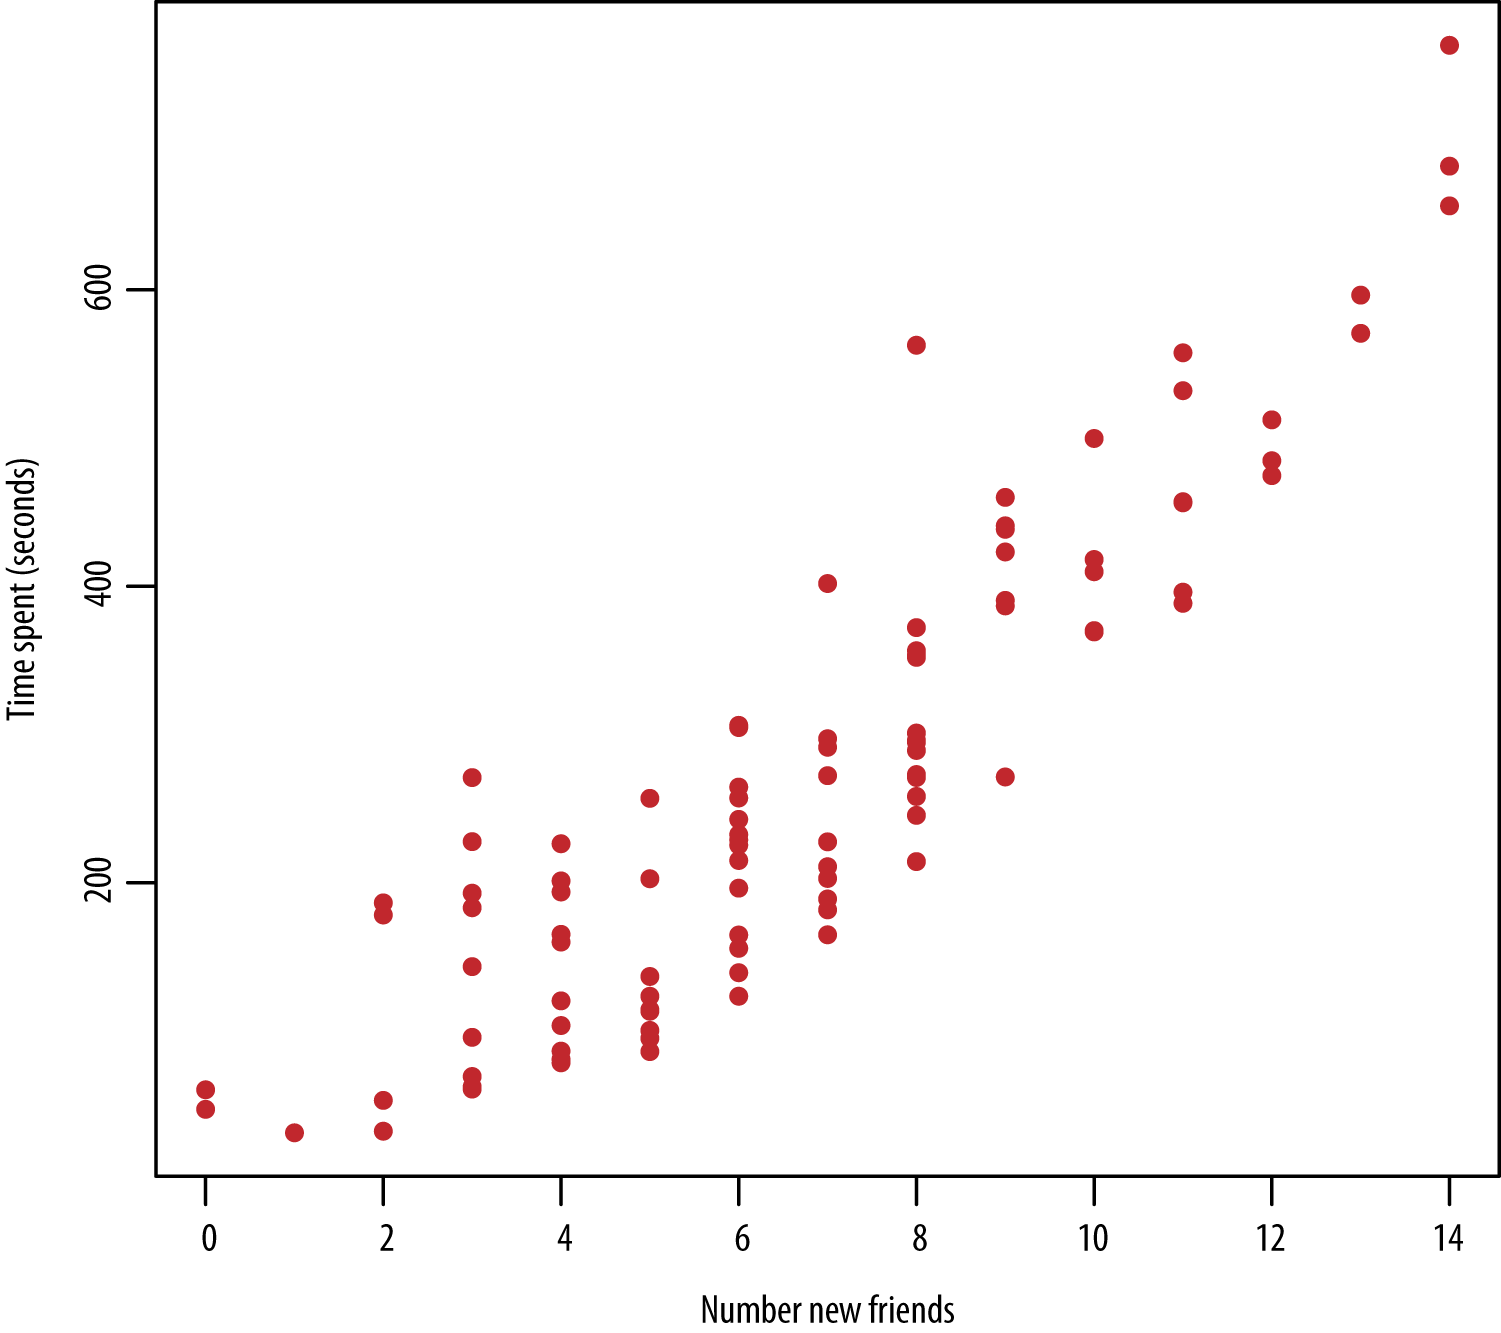
\includegraphics[width=0.7\linewidth]{imgs/fundamental_algo/algo_2.png}
    \caption{Looking kind of linear}
    \label{fig:algo_2}
\end{figure}

The relationship looks \textit{kind of} linear. But be aware that there is no perfectly \textit{deterministic} relationship between number of new friends and time spent on the site, but it makes sense that there is an \textit{association} between these two variables.

\textbf{Building Blocks} There are two things you want to capture in the model. The first is the \textit{trend} and the second is the \textit{variation}. First, we focus on the \textit{trend}. Let's assume there exist a relationship and it is linear. There are many lines and they all look they might work (Fig.\ref{fig:algo_3}).

\begin{figure}[H]
    \centering
    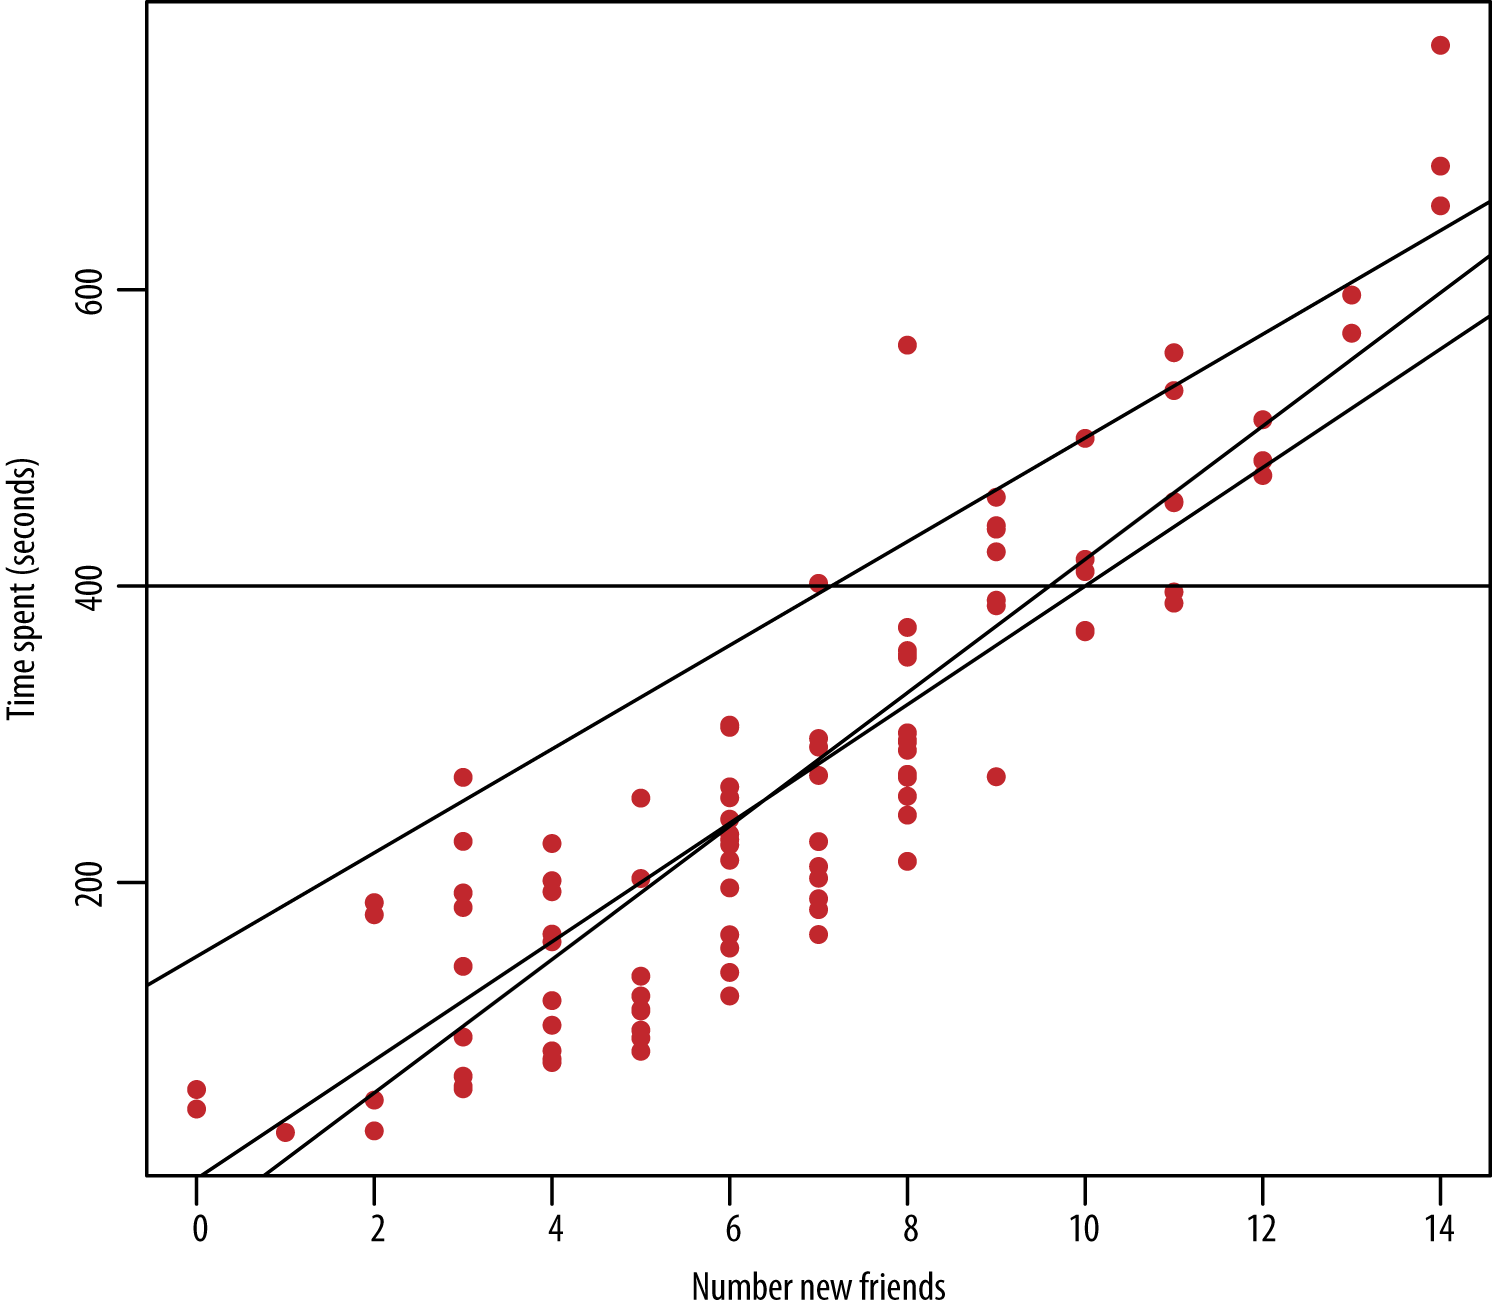
\includegraphics[width=0.7\linewidth]{imgs/fundamental_algo/algo_3.png}
    \caption{Which line is the best fit?}
    \label{fig:algo_3}
\end{figure}

Because you're assuming a linear relationship, start your model by assuming the functional form to be:
$$
    y=\beta_{0}+\beta_{1} x
$$
Now your job is to find the best choices for \(\beta_{0}\) and \(\beta_{1}\) using the observed data to estimate them: \(\left(x_{1}, y_{1}\right),\left(x_{2}, y_{2}\right), \ldots\left(x_{n}, y_{n}\right)\). Writing this with matrix notation results in this:
$$
    y=\mathbf{X} \cdot \boldsymbol{\beta}
$$
Now that we have our model, the rest is fitting the model.

\textbf{Fitting the model} The intuition behind linear regression is that you want to find the line that minimizes the distance between all points and the line. Many lines look approximately correct, but the goal is to find the optimal one. \textit{Optimal} could mean different things, but let's start with optimal to mean the line that, on average, is closest to all the points.

Linear regression seeks to find the line that minimize the sum of the squared distances between the predicted \(\widehat{y_{i}}\) s and the observed \(y_{i}\) s. This is the \textit{least squares} estimation (Fig.\ref{fig:algo_4}).
\begin{figure}[H]
    \centering
    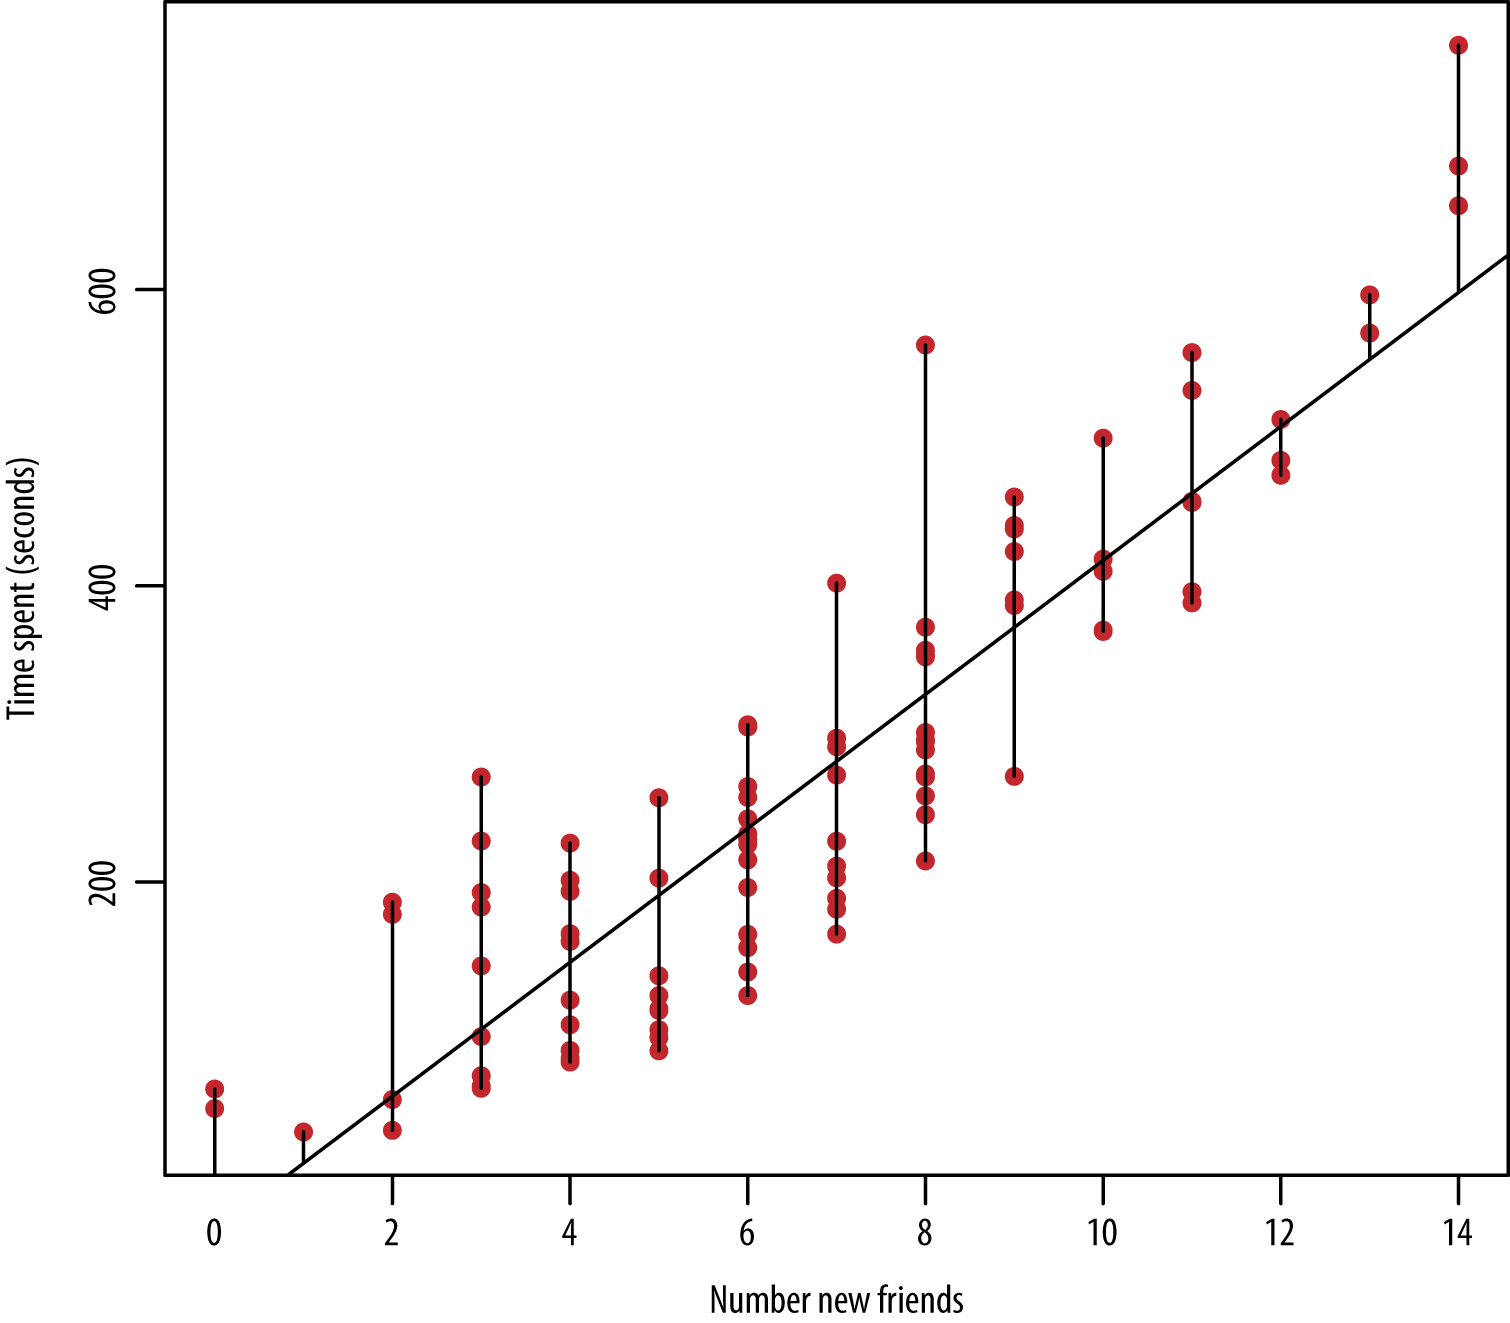
\includegraphics[width=0.7\linewidth]{imgs/fundamental_algo/algo_4.png}
    \caption{The line closest to all the points}
    \label{fig:algo_4}
\end{figure}
To find this line, you'll define the ``residual sum of squares'' (RSS) as:
\begin{equation}
    R S S(\beta)=\Sigma_{i}\left(y_{i}-\beta x_{i}\right)^{2}
    \label{eq:rss}
\end{equation}
where \(i\) ranges over the various data points. It is the sum of all the squared vertical distances between the observed points and any given line. Note this is a function of \(\beta\) and you want to optimize with respect to \(\beta\) to find the optimal line.

We have a closed solution to Eq.\ref{eq:rss}

$$
    \hat{\beta}=\left(x^{t} x\right)^{-1} x^{t} y
$$

